%%%%%%%%%%%%%%%%%%%%%%%%%%%%%%%%%%%%%%%%%%%%%%%%%%%%%%%%%%%%
%%  This Beamer template was created by Cameron Bracken.
%%  Anyone can freely use or modify it for any purpose
%%  without attribution.
%%
%%  Last Modified: January 9, 2009
%%

\documentclass[xcolor=x11names,compress]{beamer}

%%%%%%%%%%%%%%%%%%%%%%%%%%%%%%%%%%%%%%%%%%%%%%%%%%%%%%
%% General document
%%%%%%%%%%%%%%%%%%%%%%%%%%%%%%%%%%%%%%%%%%%%%%%%%%%%%%
\usepackage{graphicx}
\usepackage{tikz}
\usetikzlibrary{decorations.fractals}
% \usepackage{movie9}
% \usepackage{movie15}

% \usepackage{multicol}

% \usepackage{tabularx,ragged2e}
% \usepackage{booktabs}

\usepackage{color}

\usepackage{listings}
\lstset{ %
language=[LaTeX]TeX,
basicstyle=\normalsize\ttfamily,
keywordstyle=,
numbers=left,
numberstyle=\tiny\ttfamily,
stepnumber=1,
showspaces=false,
showstringspaces=false,
showtabs=false,
breaklines=true,
frame=tb,
framerule=0.5pt,
tabsize=4,
framexleftmargin=0.5em,
framexrightmargin=0.5em,
xleftmargin=0.5em,
xrightmargin=0.5em
}

%%%%%%%%%%%%%%%%%%%%%%%%%%%%%%%%%%%%%%%%%%%%%%%%%%%%%%
%% Beamer Layout 
%%%%%%%%%%%%%%%%%%%%%%%%%%%%%%%%%%%%%%%%%%%%%%%%%%%%%%
\useoutertheme[subsection=false,shadow]{miniframes}



%% A simple footer only with page-number
\setbeamertemplate{footline}[page number]

\setbeamertemplate{navigation symbols}{}%remove navigation symbols

\useinnertheme{default}
\usefonttheme{serif}
\usepackage{palatino}

\setbeamerfont{title like}{shape=\scshape}
\setbeamerfont{frametitle}{shape=\scshape}

\setbeamercolor*{lower separation line head}{bg=DeepSkyBlue4} 
\setbeamercolor*{normal text}{fg=black,bg=white} 
\setbeamercolor*{alerted text}{fg=red} 
\setbeamercolor*{example text}{fg=black} 
\setbeamercolor*{structure}{fg=black} 
 
\setbeamercolor*{palette tertiary}{fg=black,bg=black!10} 
\setbeamercolor*{palette quaternary}{fg=black,bg=black!10} 

\renewcommand{\(}{\begin{columns}}
\renewcommand{\)}{\end{columns}}
\newcommand{\<}[1]{\begin{column}{#1}}
\renewcommand{\>}{\end{column}}


%%%%%%%%%%%%%%%%%%%%%%%%%%%%%%%%%%%%%%%%%%%%%%%%%%%%%%
%%%%%%%%%%%%%%%%%%%%%%%%%%%%%%%%%%%%%%%%%%%%%%%%%%%%%%
%%%%%%%%%%%%%%%%%%%%%%%%%%%%%%%%%%%%%%%%%%%%%%%%%%%%%%
%%%%%%%%%%%%%%%%%%%%%%%%%%%%%%%%%%%%%%%%%%%%%%%%%%%%%%
%%%%%%%%%%%%%%%%%%%%%%%%%%%%%%%%%%%%%%%%%%%%%%%%%%%%%%
%%%%%%%%%%%%%%%%%%%%%%%%%%%%%%%%%%%%%%%%%%%%%%%%%%%%%%
%%%%%%%%%%%%%%%%%%%%%%%%%%%%%%%%%%%%%%%%%%%%%%%%%%%%%%
%%%%%%%%%%%%%%%%%%%%%%%%%%%%%%%%%%%%%%%%%%%%%%%%%%%%%%
%%%%%%%%%%%%%%%%%%%%%%%%%%%%%%%%%%%%%%%%%%%%%%%%%%%%%%
%%%%%%%%%%%%%%%%%%%%%%%%%%%%%%%%%%%%%%%%%%%%%%%%%%%%%%

\title{Study of Hydrokinetic Turbine Arrays with Large Eddy Simulation}
\subtitle{\small "fastFlume" tutorial for SOWFA}

% \author{Danny Clay Sale\\
% 		Nick Stelzenmuller\\
% 		Teymour Javaherchi\\
% 		Alberto Aliseda}

\institute{\small University of Washington, Seattle, WA, USA\\
           Dept. Mechanical Engineering\\
           Northwest National Marine Renewable Energy Center}
           

% \date{\scriptsize 67th Annual Meeting of the APS Division of Fluid Dynamics\\
%       Sunday November 23, 2014\\
%       San Francisco, California, USA}

%%%%%%%%%%%%%%%%%%%%%%%%%%%%%%%%%%%%%%%%%%%%%%%%%%%%%%
%% Main body of document
%%%%%%%%%%%%%%%%%%%%%%%%%%%%%%%%%%%%%%%%%%%%%%%%%%%%%%
\begin{document}


%%%%%%%%%%%%%%%%%%%%%%%%%%%%%%%%%%%%%%%%%%%%%%%%%%%%%%
%%%%%%%%%%%%%%%%%%%%%%%%%%%%%%%%%%%%%%%%%%%%%%%%%%%%%%
%%%%%%%%%%%%%%%%%%%%%%%%%%%%%%%%%%%%%%%%%%%%%%%%%%%%%%
%%%%%%%%%%%%%%%%%%%%%%%%%%%%%%%%%%%%%%%%%%%%%%%%%%%%%%
%%%%%%%%%%%%%%%%%%%%%%%%%%%%%%%%%%%%%%%%%%%%%%%%%%%%%%
%%%%%%%%%%%%%%%%%%%%%%%%%%%%%%%%%%%%%%%%%%%%%%%%%%%%%%
%%%%%%%%%%%%%%%%%%%%%%%%%%%%%%%%%%%%%%%%%%%%%%%%%%%%%%
%%%%%%%%%%%%%%%%%%%%%%%%%%%%%%%%%%%%%%%%%%%%%%%%%%%%%%
%%%%%%%%%%%%%%%%%%%%%%%%%%%%%%%%%%%%%%%%%%%%%%%%%%%%%%
%%%%%%%%%%%%%%%%%%%%%%%%%%%%%%%%%%%%%%%%%%%%%%%%%%%%%%
\section{\scshape Intro}

	\subsection{titlepage}
			\begin{frame}
				\titlepage
			\end{frame}

	\subsection{Focus}
		\begin{frame}{Focus}

			What is the potential power generation and environmental effects from marine hydro-kinetic (MHK) turbine farms?

			\begin{itemize}
				\item Areas to Investigate
					\begin{itemize}
						\item fluctuations of power production and structural response due to turbulence
						\item turbulence characteristics and wake evolution
						\item near field pressure fluctuations in wake
					\end{itemize}

				\item Comparison of Numerical Simulations and Experiment
					\begin{itemize}
						\item physical testing of 3 turbines in water flume
						\item large-eddy-simulation (LES) to replicate experiment
					\end{itemize}

			\end{itemize}

		\end{frame}

%%%%%%%%%%%%%%%%%%%%%%%%%%%%%%%%%%%%%%%%%%%%%%%%%%%%%%
%%%%%%%%%%%%%%%%%%%%%%%%%%%%%%%%%%%%%%%%%%%%%%%%%%%%%%
%%%%%%%%%%%%%%%%%%%%%%%%%%%%%%%%%%%%%%%%%%%%%%%%%%%%%%
%%%%%%%%%%%%%%%%%%%%%%%%%%%%%%%%%%%%%%%%%%%%%%%%%%%%%%
%%%%%%%%%%%%%%%%%%%%%%%%%%%%%%%%%%%%%%%%%%%%%%%%%%%%%%
%%%%%%%%%%%%%%%%%%%%%%%%%%%%%%%%%%%%%%%%%%%%%%%%%%%%%%
%%%%%%%%%%%%%%%%%%%%%%%%%%%%%%%%%%%%%%%%%%%%%%%%%%%%%%
%%%%%%%%%%%%%%%%%%%%%%%%%%%%%%%%%%%%%%%%%%%%%%%%%%%%%%
%%%%%%%%%%%%%%%%%%%%%%%%%%%%%%%%%%%%%%%%%%%%%%%%%%%%%%
%%%%%%%%%%%%%%%%%%%%%%%%%%%%%%%%%%%%%%%%%%%%%%%%%%%%%%
\section{\scshape Experiment}

	\subsection{Flume and Turbines}

	\begin{frame}{Tidal Turbine Reference Model 1}

		\begin{columns}
		    
		    \begin{column}{0.45\textwidth}
		        % \rule{\textwidth}{0.75\textwidth}

		        \begin{figure}[p]
				    \centering
				    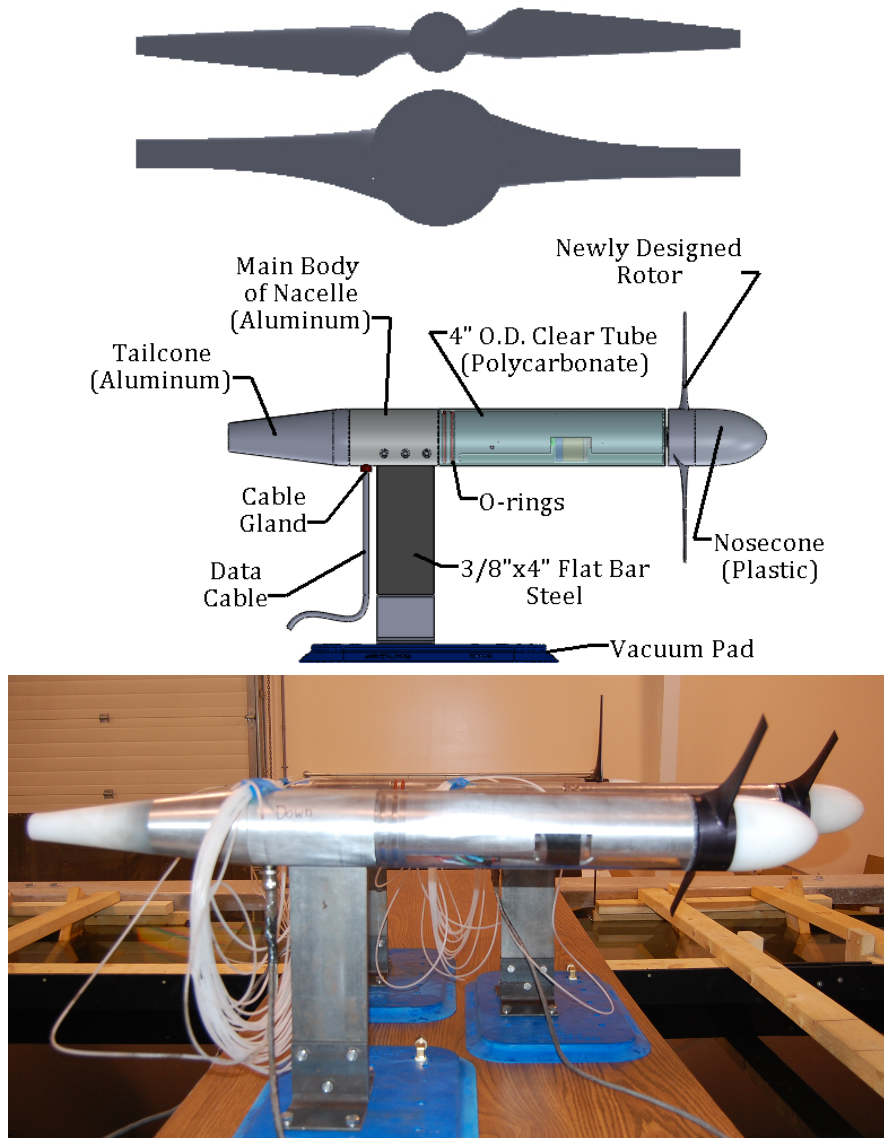
\includegraphics[width=1.1\textwidth]{figures/Nicks_turbines_redesign.png}
				    % \caption{\footnotesize lab scale turbines and flume}
				    \label{fig:Nicks turbines}
				\end{figure}

		    \end{column}
		    
		    \begin{column}{0.55\textwidth}
				
				\begin{itemize}
					\item \footnotesize horizontal-axis turbine, full-scale 550kW, diameter of 20-m
					\item created by US DOE to standardize experimental and numerical studies
					\item foils are NACA 4 and 6 series chosen for cavitation prevention and well known performance characteristics at low and high Reynolds
					\item laboratory turbine 45:1 scaling -- diameter of 45-cm
					\item attempt to match power extraction and wake characteristics at lab-scale
					\item lab-scale rotor was re-designed to minimize Reynolds scaling effects
				\end{itemize}
		    
		    \end{column}

		\end{columns}

	\end{frame}



	\begin{frame}{Flume Testing of 3 Turbines}

		\begin{figure}[p]
		    \centering
		    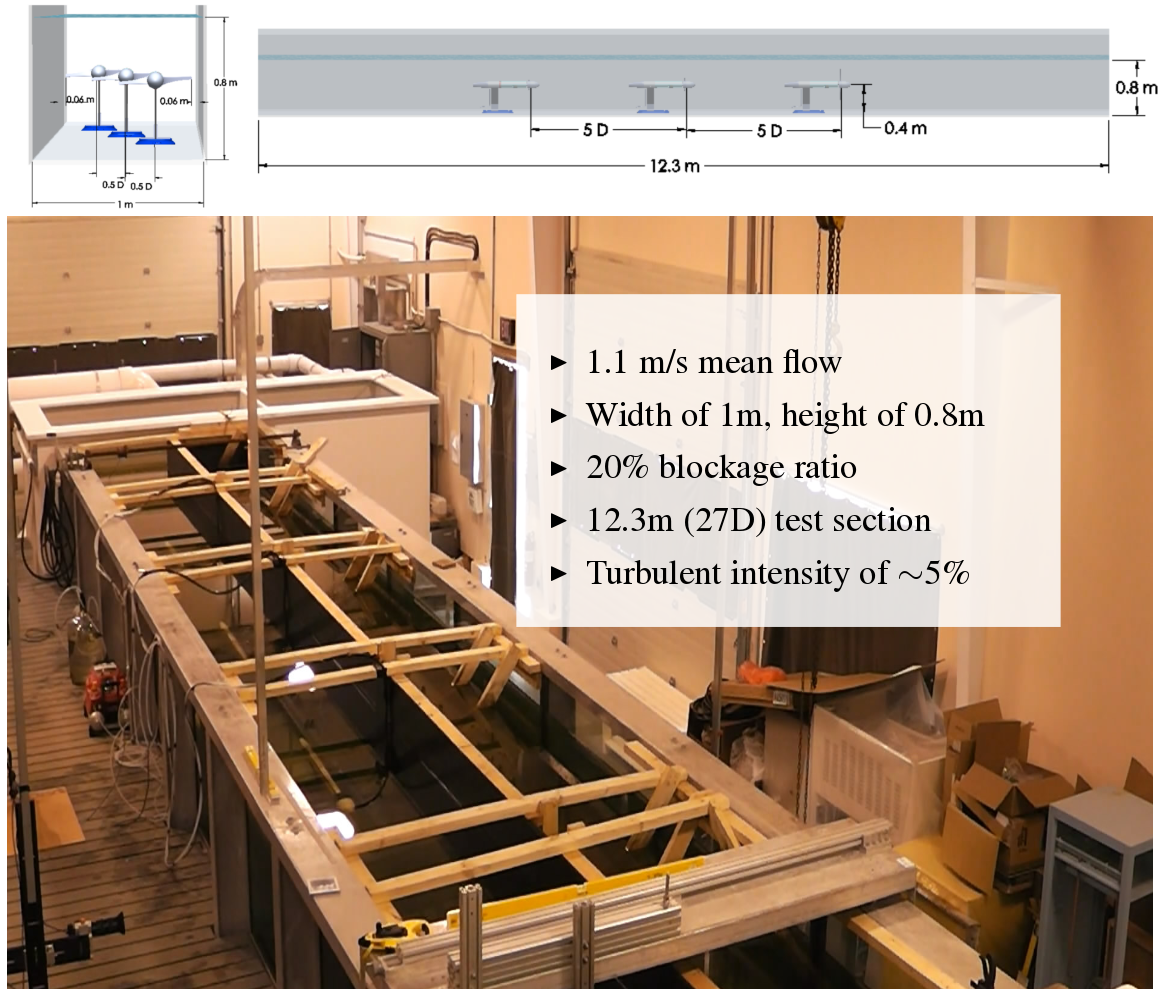
\includegraphics[width=1.0\textwidth]{figures/flume_and_description_v2.png}
		    % \caption{\footnotesize turbines in flume}
		    \label{fig:turbines in flume}
		\end{figure}


	\end{frame}

		\begin{frame}{Visualization of Tip Vortex}

		\begin{figure}[p]
		    \item bubbles are released from the nacelle to visualize tip vortex (movie)
		    \centering
		    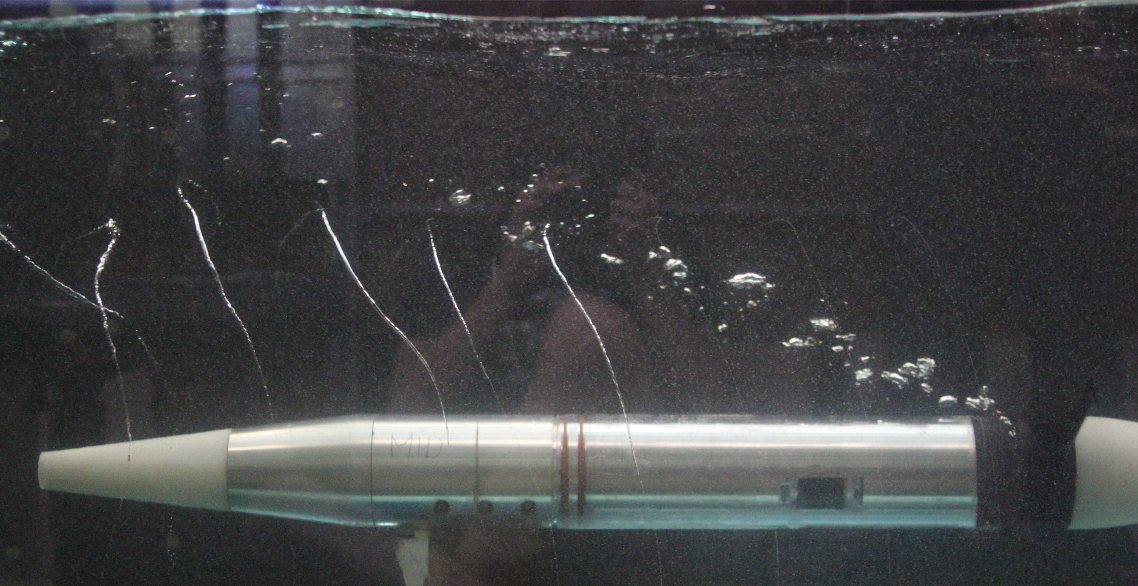
\includegraphics[width=1.0\textwidth]{figures/turbine_tip_vortex_and_bubbles.png}
		    % \caption{\footnotesize turbines in flume}
		    \label{fig:tip-vortex-and-bubbles}
		\end{figure}


	\end{frame}

%%%%%%%%%%%%%%%%%%%%%%%%%%%%%%%%%%%%%%%%%%%%%%%%%%%%%%
%%%%%%%%%%%%%%%%%%%%%%%%%%%%%%%%%%%%%%%%%%%%%%%%%%%%%%
%%%%%%%%%%%%%%%%%%%%%%%%%%%%%%%%%%%%%%%%%%%%%%%%%%%%%%
%%%%%%%%%%%%%%%%%%%%%%%%%%%%%%%%%%%%%%%%%%%%%%%%%%%%%%
%%%%%%%%%%%%%%%%%%%%%%%%%%%%%%%%%%%%%%%%%%%%%%%%%%%%%%
%%%%%%%%%%%%%%%%%%%%%%%%%%%%%%%%%%%%%%%%%%%%%%%%%%%%%%
%%%%%%%%%%%%%%%%%%%%%%%%%%%%%%%%%%%%%%%%%%%%%%%%%%%%%%
%%%%%%%%%%%%%%%%%%%%%%%%%%%%%%%%%%%%%%%%%%%%%%%%%%%%%%
%%%%%%%%%%%%%%%%%%%%%%%%%%%%%%%%%%%%%%%%%%%%%%%%%%%%%%
%%%%%%%%%%%%%%%%%%%%%%%%%%%%%%%%%%%%%%%%%%%%%%%%%%%%%%
\section{\scshape Numerical Methods}

\subsection{LES and ALM}


\subsection{LES and ALM}
\begin{frame}{}

% \vspace{-5pt}

\small The turbine model uses the 
velocity field from the LES to compute the 
hydrodynamic forces imparted on the turbine blades, and
then body forces are projected back onto flow field. \footnotemark
% \footnotetext{\tiny NWTC Information Portal (SOWFA).  https://nwtc.nrel.gov/SOWFA. Last modified 30-Sept.-2014 ; Accessed 22-Nov.-2014}
\footnotetext{\footnotesize NWTC Information Portal (SOWFA). https://nwtc.nrel.gov/SOWFA}

\vspace{-5pt}

\begin{columns}
		    
    \begin{column}{0.3\textwidth}
        % \rule{\textwidth}{0.75\textwidth}

\vspace{-10pt}

        \begin{figure}[p]
		    \centering
		    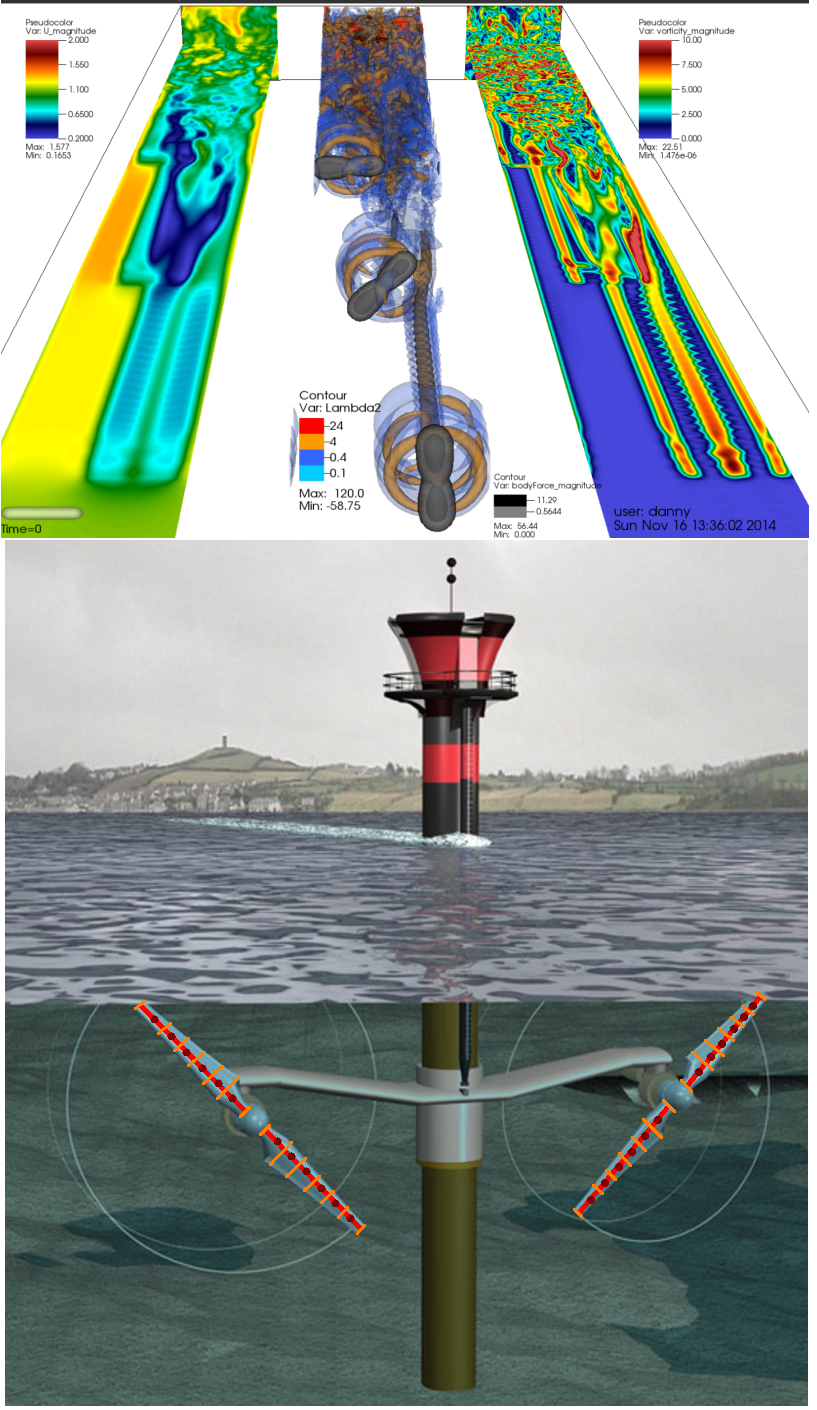
\includegraphics[width=1.1\textwidth]{figures/LES_and_cartoon_actuator_line.png}
		    % \caption{\footnotesize lab scale turbines and flume}
		    \label{fig:cartoon_actuator_line}
		\end{figure}

    \end{column}
    
    \begin{column}{0.875\textwidth}
		
		\begin{itemize}
			\item \small Large-Eddy-Simulation (LES)
			\vspace{-5pt}
				\begin{itemize}
					\item \small code: OpenFOAM (\scriptsize{Field Operation and Manipulation})
					\item second-order accurate finite-volume (FV) formulation 
					\item filter is implicitly defined by the mesh and FV discretization
					\item subgrid-stress (SGS) model is constant coefficient Smagorinsky
				\end{itemize}

			\item Actuator-Line-Method (ALM)
			\vspace{-5pt}
				\begin{itemize}
					\item \small code: FAST (\scriptsize{Fatigue Aerodynamics Structures Turbulence})
					\item creates turbulent wake and captures blade tip and root vortices
					\item similar to blade element method discretize blades into spanwise sections
					\item depends on airfoil lookup tables for lift, drag, moment, min. pressure coefficients
					\item normalized forces projected onto flow field with equal and opposite direction
				\end{itemize}

		\end{itemize}
    
    \end{column}

\end{columns}



\end{frame}



%%%%%%%%%%%%%%%%%%%%%%%%%%%%%%%%%%%%%%%%%%%%%%%%%%%%%%
%%%%%%%%%%%%%%%%%%%%%%%%%%%%%%%%%%%%%%%%%%%%%%%%%%%%%%
%%%%%%%%%%%%%%%%%%%%%%%%%%%%%%%%%%%%%%%%%%%%%%%%%%%%%%
%%%%%%%%%%%%%%%%%%%%%%%%%%%%%%%%%%%%%%%%%%%%%%%%%%%%%%
%%%%%%%%%%%%%%%%%%%%%%%%%%%%%%%%%%%%%%%%%%%%%%%%%%%%%%
%%%%%%%%%%%%%%%%%%%%%%%%%%%%%%%%%%%%%%%%%%%%%%%%%%%%%%
%%%%%%%%%%%%%%%%%%%%%%%%%%%%%%%%%%%%%%%%%%%%%%%%%%%%%%
%%%%%%%%%%%%%%%%%%%%%%%%%%%%%%%%%%%%%%%%%%%%%%%%%%%%%%
%%%%%%%%%%%%%%%%%%%%%%%%%%%%%%%%%%%%%%%%%%%%%%%%%%%%%%
%%%%%%%%%%%%%%%%%%%%%%%%%%%%%%%%%%%%%%%%%%%%%%%%%%%%%%
\section{\scshape Simulation 3 Turbines}

\subsection{3 turbines}

	% \begin{frame}{Turbines=3  TSR=6.2  Mesh=(coarse, medium)}

	% 	\begin{itemize}
	% 		\item \LARGE movie time ;-)
	% 			\begin{itemize}
	% 	            \item \tiny fastFlume  Turbines=3 TSR=6.2 Layout=offset Mesh=coarse BC=slip.gif
	% 	            \item \tiny fastFlume  Turbines=3 TSR=6.2 Layout=offset Mesh=medium BC=slip.gif
	%             \end{itemize}
 %        \end{itemize}
	% \end{frame}

	\begin{frame}{Turbines=3  TSR=6.2  Mesh=(coarse, medium)}
		
		\begin{columns}
		    
		    \begin{column}{0.6\textwidth}
		        \begin{figure}[p]
				    \centering
				    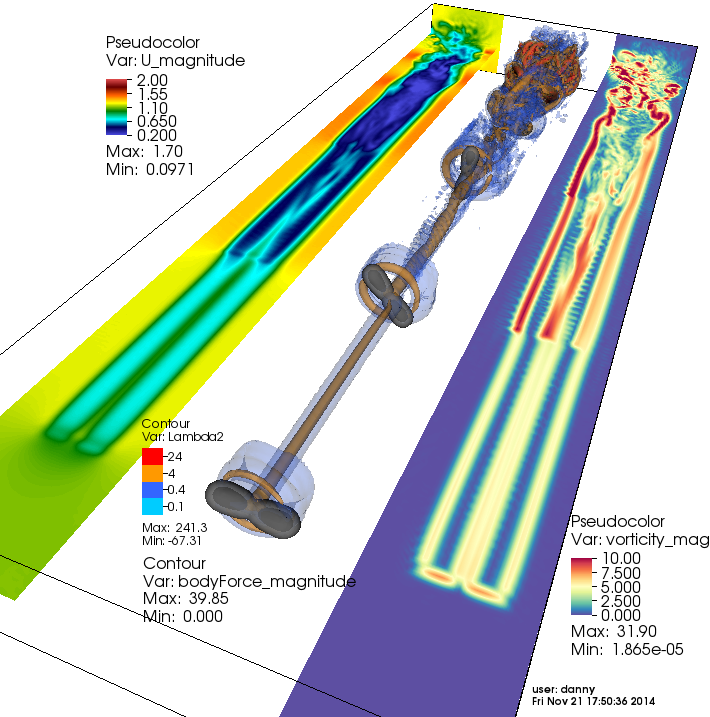
\includegraphics[width=0.8\textwidth]{figures/fastFlume-v5__Turbines=3_TSR=6p2_Layout=offset_Mesh=coarse_maxTime=10__0741.png}
				    % \caption{\footnotesize coarse mesh (465x50x40), \Delta x = 0.020 m, TSR = 6.2}
				    \caption{\scriptsize{coarse mesh 465x50x40, dx = 0.020 m}}
				    % \label{coarse mesh (465x50x40), slip-BC, TSR 6.2}
				\end{figure}

		    \end{column}
		    
		    \begin{column}{0.6\textwidth}
		        \begin{figure}[p]
				    \centering
				    % \includegraphics[width=0.8\textwidth]{figures/fastFlume-v6__Turbines=3_TSR=6p2_Layout=offset_Mesh=medium_maxTime=3p72__0183.png}
				    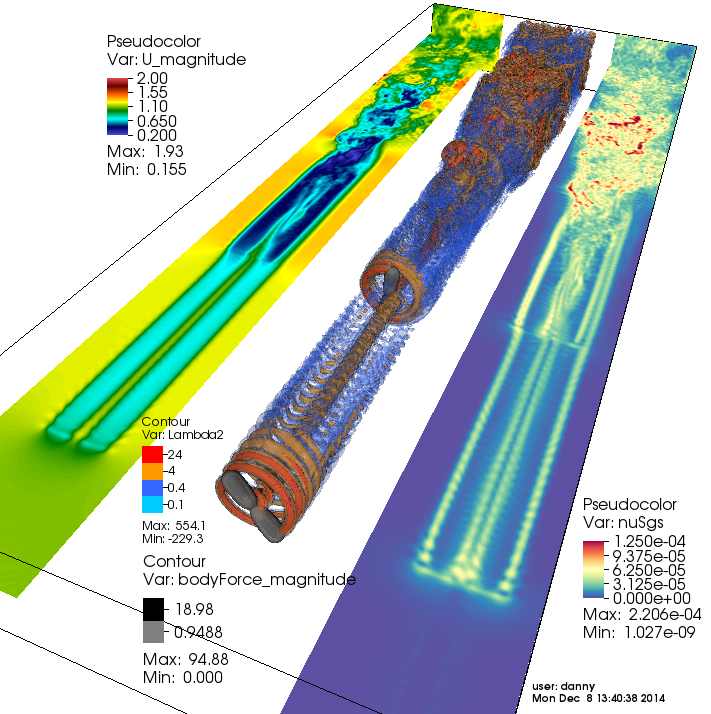
\includegraphics[width=0.8\textwidth]{figures/fastFlume-v6__Turbines=3_TSR=6p2_Layout=offset_Mesh=medium_maxTime=10.png}
				    % \caption{\footnotesize medium mesh (698x75x60), \Delta x = 0.013 m, TSR = 6.2}
				    \caption{\scriptsize{medium mesh 698x75x60, dx = 0.013 m}}
				    % \label{coarse mesh (465x50x40), periodic-BC, TSR 7}
				\end{figure}

		    \end{column}

		\end{columns}

	\end{frame}

	% \begin{frame}{at higher resolution}
	% 	\begin{figure}[p]
	% 	    \centering
	% 	    \includegraphics[width=0.65\textwidth]{figures/fastFlume__Turbines=3_TSR=6p2_Layout=offset_Mesh=medium_maxTime=15_BC=slip.png}
	% 	    \caption{\footnotesize medium mesh (698x75x60), slip-BC, TSR 7}
	% 	    \label{fig:medium mesh (698x75x60), slip-BC, TSR 7}
	% 	\end{figure}
	% \end{frame}

\subsection{analysis}
	
	\begin{frame}{}
		
		\vspace{-20pt}

		\begin{figure}[p]
		    \centering
		    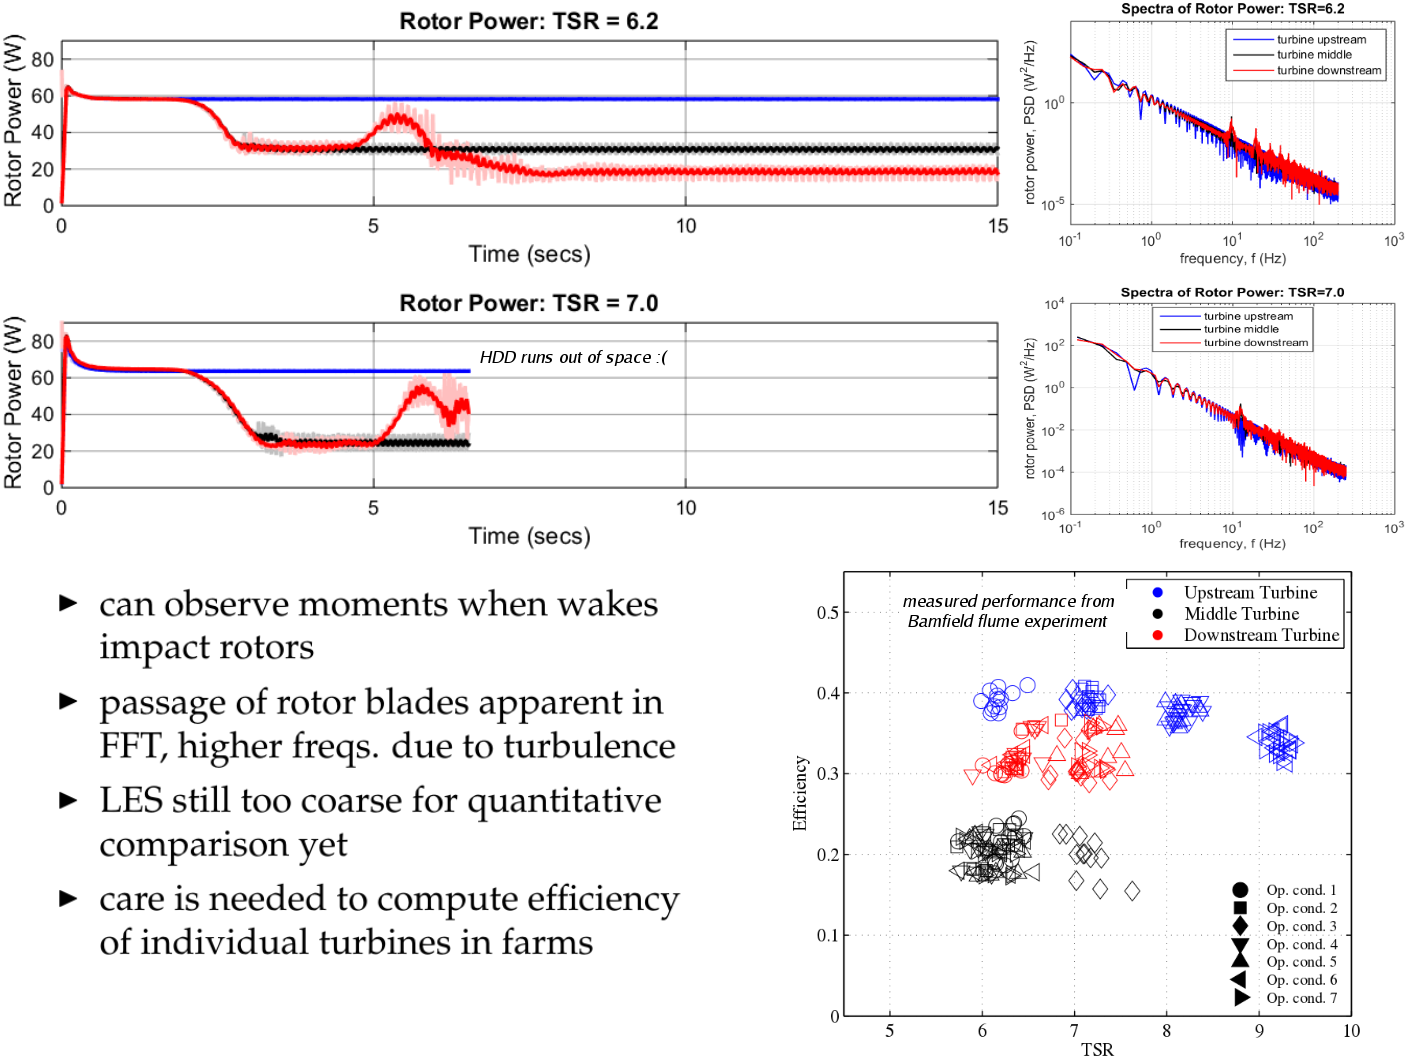
\includegraphics[width=1.090\textwidth]{figures/Analysis_Slide.png}
		    % \caption{\footnotesize medium mesh (698x75x60), slip-BC, TSR 7}
		    % \label{fig:medium mesh (698x75x60), slip-BC, TSR 7}
		\end{figure}

		  %   \begin{column}{0.6\textwidth}
		  %       % \rule{\textwidth}{0.75\textwidth}

				% \begin{itemize}
				% 	\item \small can observe moments when wakes impact rotors
				% 	\item passage of rotor blades apparent in FFT, higher freqs. due to turbulence
				% 	\item LES still too coarse for quantitative comparison yet
				% 	\item care is needed to compute efficiency of individual turbines in farms
				% \end{itemize}

		  %   \end{column}
		    


	\end{frame}

%%%%%%%%%%%%%%%%%%%%%%%%%%%%%%%%%%%%%%%%%%%%%%%%%%%%%%
%%%%%%%%%%%%%%%%%%%%%%%%%%%%%%%%%%%%%%%%%%%%%%%%%%%%%%
%%%%%%%%%%%%%%%%%%%%%%%%%%%%%%%%%%%%%%%%%%%%%%%%%%%%%%
%%%%%%%%%%%%%%%%%%%%%%%%%%%%%%%%%%%%%%%%%%%%%%%%%%%%%%
%%%%%%%%%%%%%%%%%%%%%%%%%%%%%%%%%%%%%%%%%%%%%%%%%%%%%%
%%%%%%%%%%%%%%%%%%%%%%%%%%%%%%%%%%%%%%%%%%%%%%%%%%%%%%
%%%%%%%%%%%%%%%%%%%%%%%%%%%%%%%%%%%%%%%%%%%%%%%%%%%%%%
%%%%%%%%%%%%%%%%%%%%%%%%%%%%%%%%%%%%%%%%%%%%%%%%%%%%%%
%%%%%%%%%%%%%%%%%%%%%%%%%%%%%%%%%%%%%%%%%%%%%%%%%%%%%%
%%%%%%%%%%%%%%%%%%%%%%%%%%%%%%%%%%%%%%%%%%%%%%%%%%%%%%
\section{\scshape Future Work}

\subsection{Future Work}

	\begin{frame}{Future Work}

		\begin{itemize}
			\item Code and Computers
				\begin{itemize}
					\item prototype simulations for running on more powerful hardware
					\item shared memory, distributed memory, co-processors
					\item want to understand resolution required to resolve wakes and turbine performance accurately
					\item based upon free and opensource software					
				\end{itemize}

			\item Ambient Turbulence
				\begin{itemize}
					\item turbulent structures within ambient flow can cause loading events with significance comparable to when turbines operate in upstream wakes
					\item boundary data on inlet planes generated from either precursor LES or synthetic turbulence methods (e.g. pyTurbSim)
				\end{itemize}

			\item Control Strategies
				\begin{itemize}
					\item dynamical model of rotor drivertrain to allow variable TSR as response to fluctuations in rotor torque
					\item rotor speed and pitch control for "in-water" dynamometer testing
				\end{itemize}
		\end{itemize}
	
	\end{frame}

%%%%%%%%%%%%%%%%%%%%%%%%%%%%%%%%%%%%%%%%%%%%%%%%%%%%%%
%%%%%%%%%%%%%%%%%%%%%%%%%%%%%%%%%%%%%%%%%%%%%%%%%%%%%%
%%%%%%%%%%%%%%%%%%%%%%%%%%%%%%%%%%%%%%%%%%%%%%%%%%%%%%
%%%%%%%%%%%%%%%%%%%%%%%%%%%%%%%%%%%%%%%%%%%%%%%%%%%%%%
%%%%%%%%%%%%%%%%%%%%%%%%%%%%%%%%%%%%%%%%%%%%%%%%%%%%%%
%%%%%%%%%%%%%%%%%%%%%%%%%%%%%%%%%%%%%%%%%%%%%%%%%%%%%%
%%%%%%%%%%%%%%%%%%%%%%%%%%%%%%%%%%%%%%%%%%%%%%%%%%%%%%
%%%%%%%%%%%%%%%%%%%%%%%%%%%%%%%%%%%%%%%%%%%%%%%%%%%%%%
%%%%%%%%%%%%%%%%%%%%%%%%%%%%%%%%%%%%%%%%%%%%%%%%%%%%%%
%%%%%%%%%%%%%%%%%%%%%%%%%%%%%%%%%%%%%%%%%%%%%%%%%%%%%%
% \section{\scshape Outro}

% \subsection{THANKS}
% 	\begin{frame}{Questions??? Suggestions???}

% 	\end{frame}










\end{document}